\documentclass[tikz,border=10pt]{standalone}
\begin{document}
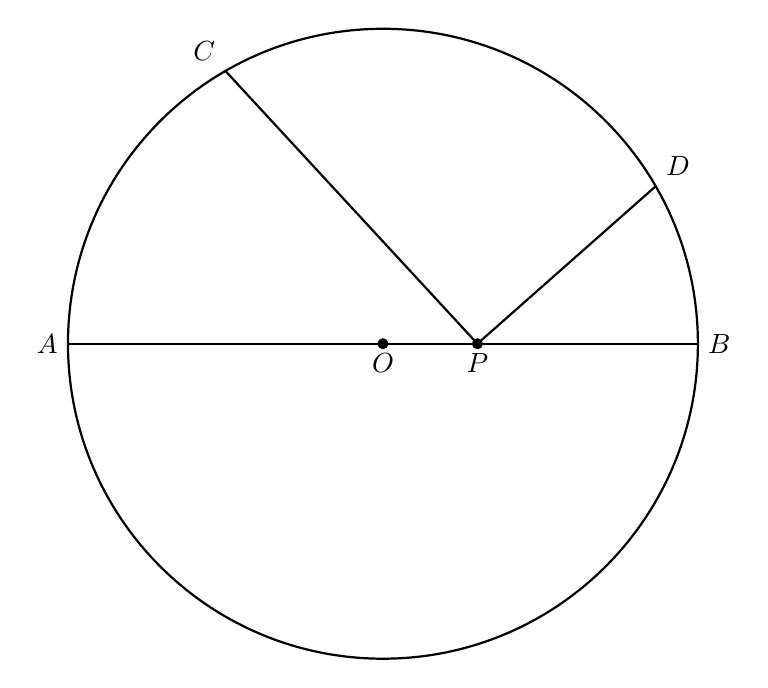
\begin{tikzpicture}[thick]
  \coordinate (O) at (0,0);
  \coordinate (A) at (-4,0);
  \coordinate (B) at (4,0);
  \coordinate (P) at (1.2,0);
  \coordinate (C) at (-2,3.4641);
  \coordinate (D) at (3.4641,2);

  \draw (O) circle (4);
  \draw (A) -- (B);
  \draw (P) -- (C);
  \draw (P) -- (D);

  \fill (O) circle (2pt);
  \fill (P) circle (2pt);

  \node[left] at (A) {$A$};
  \node[right] at (B) {$B$};
  \node[below] at (O) {$O$};
  \node[below] at (P) {$P$};
  \node[above left] at (C) {$C$};
  \node[above right] at (D) {$D$};
\end{tikzpicture}
\end{document}
